\section{Budowa aplikacji}
Prezentowana aplikacja zbudowana jest z 2 modułów:
\begin{itemize}
    \item Aplikacji obliczeniowej opartej o środowisko MPI (nazywana dla
    uproszczenia \textbf{serwerem})
    \item Aplikacja z interfejsem graficznym (nazywana dla uproszczenia
    \textbf{klientem})
\end{itemize}

Moduły te komunikują się ze sobą za pomocą \textbf{potoków nazwanych}. Jeden z
tych potoków odpowiada za przekazywanie poleceń do serwera, a drugi za odsyłanie
wygenerowanych na podstawie żądania danych w drugą stronę.

\subsection{Interfejs komunikacyjny}
\subsubsection{Klient $\rightarrow$ Serwer}
Struktura \ref{Request} opisuje dane przekazywane do serwera.
\begin{itemize}
    \item \textit{connectionOk} sygnalizuje czy interfejs użytkownika jest
    aktywny. Wartość \textbf{fałsz} oznacza że aplikacja powinna zostać
    zamknięta.
    \item Pola \textit{windowHeight} oraz \textit{windowWidth} przechowują
    informację o wysokości i szerokości okna wyrażonej w ilości pikseli.
    \item Pozostałe pola przechowują informację o punktach w przestrzeni
    zespolonej pomiędzy którymi ma zostać wyznaczony zbiór Mandelbrota.
\end{itemize}
\begin{figure}[H]
\begin{minted}
    [frame=lines, framesep=2mm, baselinestretch=1.2, fontsize=\footnotesize,linenos] {c++}

struct Request {
    bool connectionOk; 
    int windowWidth; 
    int windowHeight; 
    double leftTopX; 
    double leftTopY; 
    double rightBottomX; 
    double rightBottomY;
};   
\end{minted}
\captionof{listing}{Struktura opisująca zapytanie do serwera}
\label{Request}
\end{figure}

\newpage
\subsubsection{Serwer $\rightarrow$ Klient}
Serwer w odpowiedzi na zapytanie wysyła dane, które interpretowane są jako obraz
do wyświetlenia.

\begin{figure}[H]
\begin{minted}
    [frame=lines, framesep=2mm, baselinestretch=1.2, fontsize=\footnotesize, linenos] {c++}
struct Pixel {
    uint8_t R; 
    uint8_t G; 
    uint8_t B;
};

struct Response {
    Pixel img[windowWidth*windowHeight];
};   
\end{minted}
\captionof{listing}{Struktura opisująca odpowiedź serwera}
\label{Response}
\end{figure}

Dane przedstawione na listingu \ref{Response} stanowią reprezentację obrazu w
postaci jednowymiarowej tablicy bajtów. Aby zrekonstruować taki strumień danych
należy odczytywać każdy piksel po kolei, a następnie wypełniać obraz wierszami z
góry na dół, od lewej do prawej.\\

Kolor kodowany jest w przestrzeni kolorów RGB.

\begin{figure}[H]
    \centering
    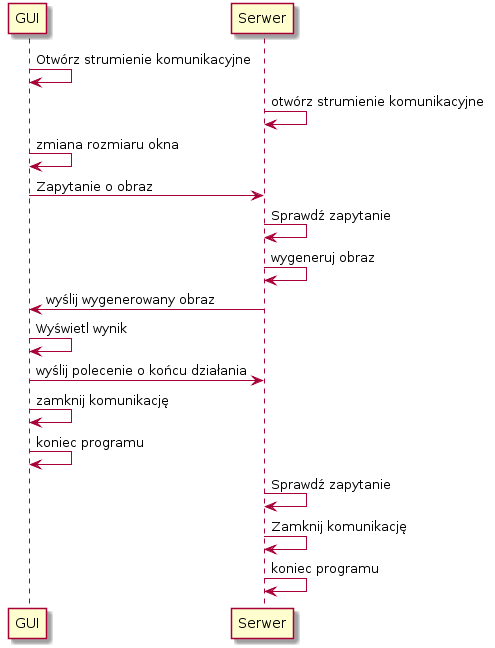
\includegraphics[width = 0.7\textwidth]{img/diagram.png}
\end{figure}
\subsection{Serwer}
Zasada podziału pracy w części serwerowej przedstawiona jest na poniższym
diagramie. Obraz dzielony jest na linie grubości 1 px. Każdy wątek poza wątkiem
głównym dostaję za zadanie obliczenie lini. Wątek główny ma za zadanie zebrać
wszystkie wyliczone linie obrazu w odpowiedniej kolejności. Kiedy obraz zostanie
w pełni wygenerowany wątek główny który jest również odpowiedzialny za
komunikację z GUI wysyła gotowy obraz do użytkownika. Taka struktura podziału
pracy sprawia że serwer musi działać \textbf{przynajmniej na 2 wątkach},
ponieważ wątek główny odpowiedzialny jest za komunikację oraz łączenie obrazu w
całość, natomiast pozostałe wątki odpowiadają wyłącznie za generowanie danych.
\begin{figure}[H]
    \centering
    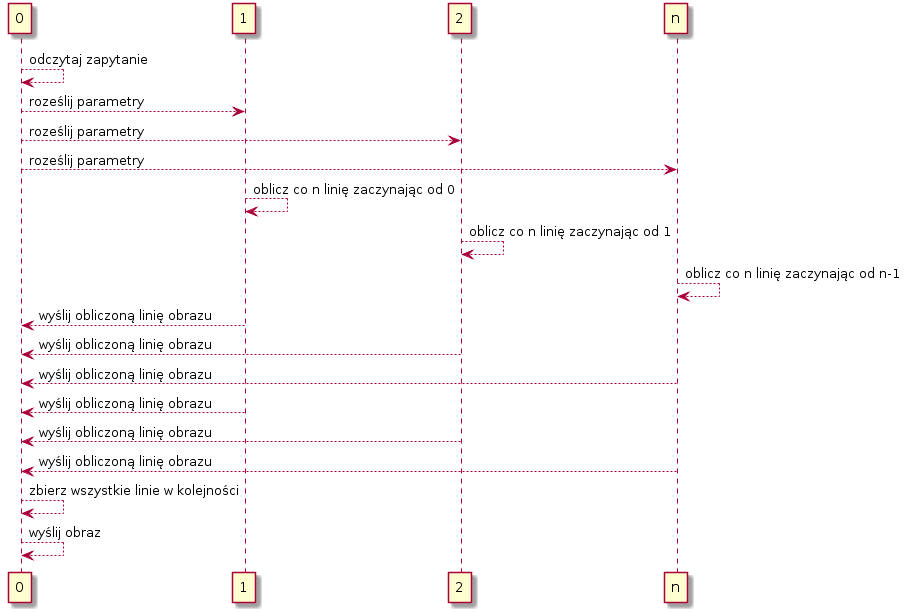
\includegraphics[width = \textwidth]{img/watki.png}
\end{figure}

Algorytm wyznaczania zbioru Mandelbrota opiera się na podnoszeniu do kwadratu
liczby zespolonej i dodawaniu do niej stałej. Jeśli wartość tej liczby po
podniesieniu do kwadratu jest mniejsza od 2, istnieje szansa, że punkt ten
należy do zbioru. Aby to potwierdzić uzyskaną wartość ponownie podnosi się do
kwadratu i dodaje tę samą stałą. Jeśli po odpowiednio dużej ilości iteracji
wartość ta nie przekroczy 2, to punkt uznaje się za część zbioru, jeśli jednak
wartość ta przekroczy 2, to dla danego punktu wybierany jest odpowiedni kolor w
zależności od ilości iteracji przez które ten punkt miał wartość poniżej 2.

Prezentowany algorytm jest więc bardzo niezależny. Teoretycznie nie ma przeszkód
aby każdy piksel liczony był niezależnie, jednak ze względu na prostotę
implementacji, oraz łatwość rekonstrukcji obrazu, każdy wątek na raz liczy
jedynie linię szerokości grubości 1 px i szerokości docelowego obrazu.

\subsection{GUI}
Interfejs użytkownika po połączeniu do serwera wysyła pierwsze zapytanie o
wygenerowanie obrazu zbioru Mandelbrota.

Możliwa jest zmiana rozmiaru okna, oraz przybliżania części obrazu. W trakcie
zaznaczania trzymając lewy przycisk myszy obszaru do przybliżania zachowywane są
proporcje ekranu.

Zaimplementowana została również funkcja cofania przybliżenia realizowana za
pomocą prawego przycisku myszy.

Należy zwrócić uwagę, że dość łatwo jest zbliżyć się w takim stopniu do elementu
obrazu że wartości szerokość okna na płaszczyźnie zespolonej nie może być
dokładnie wyznaczona za pomocą liczby zmiennoprzecinkowej, a przy znacznym
przybliżeniu obliczenia mogą zająć znacząco dłużej ze względu na konieczność
zwiększania ilości iteracji dla każdego piksela, aby zachować ostre krawędzie
oraz odpowiednią paletę kolorów poza zbiorem.

\section{Sposób użycia}

\subsection{Wymagania}
\begin{itemize}
    \item Biblioteka SDL2 (klient)
    \item Środowisko MPI (serwer)
    \item System UNIX lub UNIXopodobny wspierający POSIX
    \item Serwer X
    \item Program pkg-config
    \item Program GNU Make
    \item Kompilator języka C++ kompatybilny ze standardem C++11 lub wyższym
\end{itemize}

\subsection{Kompilacja i konsolidacja}
Proces kompilacji i uruchomienia jest zautomatyzowany poprzez system budowania Make lub CMake.
Domyślnie używany jest kompilator i konsolidator dostarczany w ramach projektu GNU GCC.\\

Dostarczone są dwa pliki Makefile
\begin{itemize}
    \item [A] \textbf{Makefile} -- zakładający, że biblioteka SDL2 i środowisko
    MPI jest na danej platformie zainstalowane. Odpowiednie ścieżki do nagłówków
    i bibliotek znajdowane są poprzez program \textit{pkg-config}.
    \item [B] \textbf{MakefileShippedSDL} -- korzystający z biblioteki dynamicznej i
    nagłówków dostarczonych wraz z repozytorium kodu. Dostarczona biblioteka
    zakłada wykorzystanie na platformie zaopatrzonej w dystrybucję Debian w
    wersji Stretch. 
\end{itemize}

Dostępne cele w ramach Make
\begin{itemize}
    \item \textbf{all} -- zbuduj wszystkie aplikacje (target/ClientMandelbrot
    oraz target/ServerMandelbrot)
    \item \textbf{clean} -- wyczyść katalog repozytorium (usuwa target oraz build)
    \item \textbf{run\_local} -- Uruchamia kompletną aplikację: Startuje
    równolegle klienta i serwer w środowisku MPI wykorzystując wszystkie rdzenie
    fizyczne danej platformy.
\end{itemize}

\subsection{Uruchomienie aplikacji}
Można uruchomić aplikację wykorzystując jedynie bieżącą maszynę za pomocą
\begin{itemize}
    \item \textit{\$ make run\_local -j} -- dla wariantu A makefile
    \item \textit{\$ make -f MakefileShippedSDL run\_local -j} -- dla wariantu B makefile
\end{itemize}

Aby uruchomić ją na wielu komputerach jednocześnie należy manualnie wygenerować
plik zawierający nazwy komputerów dostępnych w sieci LAN poprzez protokół SSH i
uruchomić serwer za pomocą adekwatnej dyrektywy \textit{mpiexec}.

\subsection{Obsługa klienta}
Po uruchomieniu aplikacji (tj. poprawnym uruchomieniu klienta i serwera) pojawia
się graficzna interpretacja zbioru Mandelbrota na płaszczyźnie zespolonej w
przedziałach dla osi X: $[-2, 0.5]$ i Y: $[-1.5, 1.5]$. Okno programu uruchamia
się domyślnie zachowując proporcje płaszczyzny. Zmiana rozmiaru okna
\textbf{zaburza proporcje} -- jest to zachowanie oczekiwane.

Sterowanie:
\begin{itemize}
    \item \textbf{Naciśnięcie lewego przycisku myszy, przeciągnięcie kursorem po
    ekranie, a następnie puszczenie} -- \\
    powoduje wypełnienie ekranu zbiorem z zaznaczonego przedziału. Powoduje to
    wywołanie zapytania do serwera o przeprowadzenie obliczeń.
    \item \textbf{Naciśnięcie prawego przycisku myszy} -- \\
    Wraca do poprzedniego zestawu koordynatów zespolonych wyświetlanych przez klienta.
    \item \textbf{Zamknięcie okna} -- \\
    Zamyka program i serwer w sposób zdefiniowany, wraz ze zamknięciem potoków i
    usunięciem ich reprezentacji plikowych.
\end{itemize}